\documentclass{article}
\usepackage[T1]{fontenc}
\usepackage{lmodern}
\usepackage{graphicx}
\usepackage{amsmath,amssymb}
\usepackage[a4paper,margin=2cm]{geometry}
\usepackage[absolute,overlay]{textpos}
\setlength{\TPHorizModule}{1mm}
\setlength{\TPVertModule}{1mm}
\usepackage[indonesian]{babel}
\usepackage{hyperref}
\setlength{\emergencystretch}{2em}
% unit: Halaman 52

\begin{document}

% === Halaman 52 (llm) ===

\section*{Dekripsi}

\vspace{10mm}

\begin{minipage}[t]{0.45\textwidth}
\begin{verbatim}
//Dekripsi sembarang berkas dengan algoritma RC4
#include <iostream>
#include <string.h>
#include <stdlib.h>
#include <stdio.h>
using namespace std;

main(int argc, char *argv[])
{
 FILE *Fin, *Fout;
 char p, c, u;
 string K;
 int S[256];
 int i, j, t;
\end{verbatim}
\end{minipage}
\hfill
\begin{minipage}[t]{0.45\textwidth}
\begin{verbatim}
Fin = fopen(argv[1], "rb");
if (Fin == NULL) {
 cout << "Berkas " << argv[1] <<" tidak ada" << endl;
 exit(0);
}

Fout = fopen(argv[2], "wb");

cout << "Kata kunci : "; cin >> K;
cout <<"Dekripsi " << argv[1] << " menjadi " << argv[2] << "...";

for (i = 0; i<256; i++){
 S[i] = i;
}
\end{verbatim}
\end{minipage}

% deskripsi: Screenshot potongan kode program C++ untuk proses dekripsi menggunakan algoritma RC4 yang terbagi dalam dua kolom.
% bbox normalisasi: [0.0400, 0.1800, 0.9800, 0.7800]
\begin{textblock*}{197.40mm}(8.40mm,53.46mm)
\noindent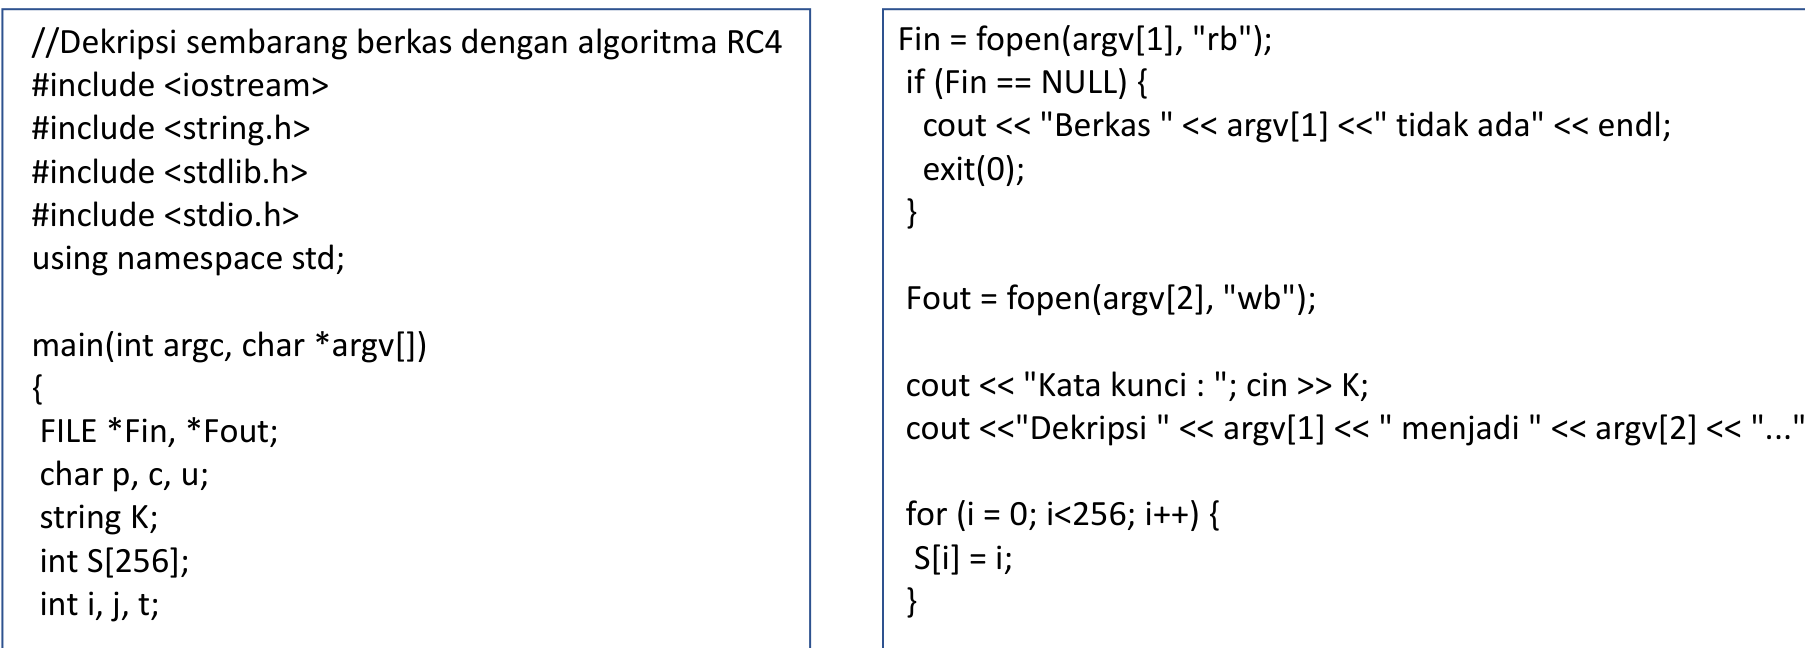
\includegraphics[width=197.40mm,height=178.20mm]{../../images/llm/page_052_img_01.png}%
\end{textblock*}

\end{document}
